\documentclass[11pt, oneside]{article}   	% use "amsart" instead of "article" for AMSLaTeX format
\usepackage[margin=1 in]{geometry}                		% See geometry.pdf to learn the layout options. There are lots.
\geometry{letterpaper}                   		% ... or a4paper or a5paper or ... 
%\geometry{landscape}                		% Activate for rotated page geometry
%\usepackage[parfill]{parskip}    		% Activate to begin paragraphs with an empty line rather than an indent
\usepackage{graphicx}				% Use pdf, png, jpg, or eps§ with pdflatex; use eps in DVI mode
								% TeX will automatically convert eps --> pdf in pdflatex		
\usepackage{amssymb}

\usepackage{amsmath}

\usepackage{url}
\usepackage{hyperref}

\newtheorem{proposition}{Proposition}
\newtheorem{example}{Example}

\usepackage{listings}
%SetFonts

%SetFonts
\usepackage{xcolor}
\usepackage{float}

\title{\vspace{-.3 in} Running In Circles}
\author{Nick Arnosti}
\date{August 6, 2018}							% Activate to display a given date or no date

\begin{document}
\maketitle
%\section{}
%\subsection{}


%\section{Motivation}

\begin{figure}
\centerline{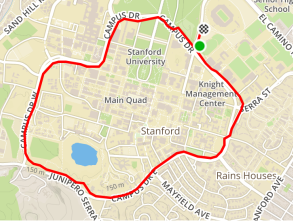
\includegraphics[width = .5 \textwidth]{campus-drive}}
\caption{Campus Drive Loop at Stanford University.}
\label{fig:campusdrive}
\end{figure}

One popular run on the Stanford campus is Campus Drive Loop. There are sidewalks on either side of the road, giving the runner a choice of which to take. On days when I felt low-energy, I would sometimes take the inside sidewalk, figuring that this would shorten my run. But by how much?

If the loop were a perfect circle, the answer would be easy -- my savings would be $2 \pi$ times the width of the road, implying a shorter route by something like 300 ft. But as shown in Figure \ref{fig:campusdrive}, the loop is far from circular, and is not even convex. I wondered, is 300 feet still a reasonable answer, or is it possible that the savings could be much more or much less?

After drawing a few simple shapes (mostly compositions of straight lines and partial circles), I became convinced that in fact, the answer was $2\pi$ times the width of the road, regardless of its shape. But I felt I lacked the tools to tackle the problem formally. This is where my friend Jake Levinson comes in. I posed this question to him while on Safari in Tanzania, and he promptly tackled it with gusto (see Figure \ref{fig:safari}).

%It turns out that there are some subtleties to the problem 





\begin{figure}
\centerline{\includegraphics[width = .5 \textwidth]{math} \hspace{.05 in} \includegraphics[width = .5 \textwidth]{safari}}
\caption{Left: Jake sketching ideas in a cafe in Moshi. Right: how we spent the rest of our time.}
\label{fig:safari}
\end{figure}

\end{document}  